\documentclass{article}
\usepackage{graphicx}
\usepackage{amsmath,amssymb}
\usepackage{hyperref}
\title{Numerical analysis of k-means initializations}
\author{Bijan Varjavand}
\date{\today}
\begin{document}
\maketitle
\section{Abstract}
Many people use k-means for clustering, but are unaware of how exactly they should run the algorithm, and with which parameters.
We find considerations when evaluating one's choice of initialization, and suggest parameterizations which offer a suitable middle ground.
We've found that k-means simply initialized once randomly and allowed to converge performs poorly, while using k-means++ initialization greatly improves the accuracy but takes longer.
Using additional initializations and choosing the best initialization to start gives diminishing returns and is use scales with the complexity of the data.

\section{Intro}
Finding a global minimum for a clustering problem is NP-hard for even 2 clusters in d dimensions. K-means is a commonly used approximation algorithm to solve this problem.

\subsection{Data}
Let $X|Y \sim Normal(Y,\Sigma)$, $Y \in \{0,1\}$

Where
\[\Sigma = \begin{bmatrix}\sigma^2 & 0 & \dots\\0 & \sigma^2 & 0\\\dots&0&\sigma^2\end{bmatrix}, \sigma^2 = 0.5\]

The cluster sizes are balanced, so $\pi_1 = \pi_2 = 0.5$

The Bayes' optimal classifier is the best performance classifier if the true labels are known. Our data are drawn from 2 multivariate distributions $x_1,x_2 \in X$ such that the data vector is 2n long, with the final set being

$$\{x_{11}, x_{12}, \dots, x_{1n}, x_{21}, x_{22}, \dots, x_{2n}\}$$

The true class labels for the drawn data are a vector $Y$ of length $2n$ with $n$ 0s and $n$ 1s.

For a set of functions $f \in \mathcal{F}$ which are suitable for the problem, the bayes optimal is simply represented as

\begin{align*}
    f^*(x) &= \underset{f \in \mathcal{F}}{argmax} [P(f(x)=y)]\\
    &= \underset{y}{argmax} [f_{X,Y}]\\
    &= \underset{y}{argmax} [f_{X|Y}f_Y]
\end{align*}

The loss of a classifier is just the expected difference between the prediction,

$$L = E[f(X) \neq Y]$$

The Bayes optimal loss is just the loss of the Bayes classifier

\begin{align*}
    L^* &= P(f^*(X) \neq Y)
\end{align*}

In the two-class case, with equal priors,

\begin{align*}
    L^* &= P(f^*(X)=1|Y=0)P(Y=0) + P(f^*(X)=0|Y=1)P(Y=1)\\
    &= \frac{1}{2}\Big(P(f^*(X)=1|Y=0)+P(f^*(X)=0|Y=1)\Big)
\end{align*}

Observing that the probabilities in our example are equal because the distributions are symmetric

$$(P(f^*(X)=1|Y=0) = P(f^*(X)=0|Y=1))$$

\begin{align*}
    L^* &= P(f^*(X)=1|Y=0) = P(f^*(X)=0|Y=1)\\
    &= \int_{-\infty}^{\frac{1}{2}} N(1,1/2)\,dx = \int_{\frac{1}{2}}^\infty N(0,1/2)\,dx
\end{align*}

Which is just a cdf.

\begin{align*}
    P(X < \frac{1}{2}) &= P(N(1,0.5) < \frac{1}{2})\\
    &= P(0, 0.5) < -\frac{1}{2})\\
    &= P(N(0,1) < -\frac{1}{2\sqrt{0.5}})\\
    &= \Phi(-\frac{1}{2\sqrt{0.5}})\\
    &= 0.2398
\end{align*}

\begin{figure}[!ht]
  \centering
  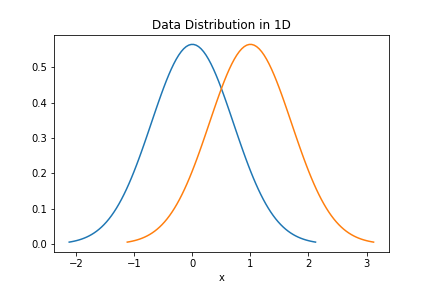
\includegraphics[scale=0.5]{bayes.png}
  \caption{The Bayes Loss of the clustering problem in one dimension}
\end{figure}

\section{Convergence to local minima}
Once the k-means algorithm has been initialized, either Lloyd's algorithm or Hartigan's algorithm are commonly used to converge to a local minima. It has been shown previously that the local minima that Hartigan's algorithm finds is a subset of those that Lloyd's algorithm finds. For the sake of simplicity we observe the behavior of the EM step with Lloyd's, but one could infer that the behavior would be similar for Hartigan's.

\subsection{High Efficiency of the EM Step}
The expectation maximization step is highly efficient when compared to initialization of the k-means algorithm.

\begin{figure}[!ht]
  \centering
  \includegraphics[scale=0.5]{em_step.png}
  \caption{allowing convergence vs not}
\end{figure}

We can see that one hypothesis of simply initializing k-means multiple times with k-means++ and choosing the best initialization doesn't perform well.

\subsection{Iterating to a local minima at higher dimensions}
Observing that it is necessary to iterate to a local minima after initialization, we observe how much effort is necessary as the dimensionality of the data increases.

\begin{figure}[!ht]
  \centering
  \includegraphics[scale=0.5]{em_step.png}
  \caption{allowing convergence vs not}
\end{figure}

It can be seen that, in higher dimensions, the clustering problem becomes more complex and the initializations are somewhat far away from a local minima. Here we can see that kmeans++ initialization lands us far closer to a local minima than simply random initialization.

\section{Choosing best initialization of n inits}
The problem we then concern ourselves with is, given some data, how much effort should be put into initialization of the k-means center seeds? We test performance of the k-means algorithm with different initialization schemas.

\subsection{Suggested Initialization Schemas}
After our numerical analysis we find that some simple benchmarks are a single k-means++ initialization, choosing the best out of 2 k-means++ initializations, and choosing the best out of 10 k-means++ initializations. Adding a second k-means++ initialization surprisingly results in a better result while sacrificing little computation/time.

\begin{figure}[!ht]
  \centering
  \includegraphics[scale=0.5]{n_inits.png}
  \caption{The time and error with increasing inits}
\end{figure}

There is a clear tradeoff here between time and error. The tradeoff itself is determined by the complexity of the data, and how much effort needs to be done to reach a local minima of satisfactory quality. A simple diagram like the one below can provide some suggestion for which initialization scheme should be used.

\begin{figure}[!ht]
  \centering
  \includegraphics[scale=0.5]{n_inits.png}
  \caption{The time and error with increasing inits}
\end{figure}

\section{Conclusion}
The behavior of k-means is highly dependent on the data, as well as how parameters of the algorithm itself are tuned. It is suggested that, if the data is simple, then a simple random initialization performs best. If the data is more complicated, with a somewhat large dimension ($>50$), using the best of 2 k-means++ initializations is preferred in order to reach more optimal local minima. If the data has incredibly high dimension ($>200$), using the best of 10 k-means++ initializations takes a long time but results in much better performance in terms of error.

\section{Appendix}
The code for numerical analysis of these experiments are located in a public reposity in \hyperlink{http://github.com/wow}{github}: 



\end{document}
